%\documentclass{standalone}
%\usepackage[utf8]{inputenc}
%\usepackage{graphicx}
%\usepackage{xcolor}
%\usepackage{pgf,tikz}
%\usepackage{mathrsfs}
%\usetikzlibrary{shapes, calc, shapes, arrows, math, babel, positioning}
%
%\begin{document}

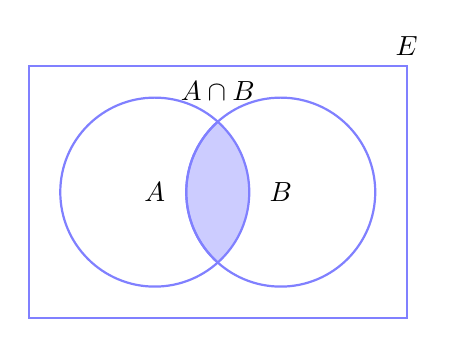
\begin{tikzpicture}[scale=0.8]
	\draw[draw=blue!50, thick] (-2,-2) rectangle (4,2) node[above] {$E$};
    \begin{scope}
        \clip (0,0) circle (1.5cm);
        \fill[fill=blue!20, draw=blue!50, thick] (0:2cm) circle (1.5cm);
    \end{scope}
    \draw[draw=blue!50, thick] (0,0) circle (1.5cm) node {$A$};
    \draw[draw=blue!50, thick] (0:2cm) circle (1.5cm) node {$B$};
    %\node[anchor=south] at (current bounding box.north) {$A \cap B$};
    \node[anchor=south] at (1,1.3) {$A \cap B$};
\end{tikzpicture}

   


% Original:
%\def\firstcircle{(0,0) circle (1.5cm)}
%\def\secondcircle{(0:2cm) circle (1.5cm)}
%\def\espacio{(-2,-2) rectangle (4,2)}
%
%\colorlet{circle edge}{blue!50}
%\colorlet{circle area}{blue!20}
%
%\tikzset{filled/.style={fill=circle area, draw=circle edge, thick},
%    outline/.style={draw=circle edge, thick}}
%    
%\begin{tikzpicture}[scale=0.8]
%\draw[outline] \espacio node[above] {$E$};
%    \draw[filled] \firstcircle node {$A$}
%                  \secondcircle node {$B$};
%    \node[anchor=south] at (1,1.3) {$A \cup B$};
%\end{tikzpicture}

%
%\end{document}